%!TEX TS-program = xelatex
%!TEX encoding = UTF-8 Unicode
\documentclass[a4paper, 12pt, oneside]{book}

\usepackage{cite}
%\usepackage{chapterbib}
%The chapterbib package facilitates multiple bibliographies in a LATEX document
\usepackage[hyphens]{url}
%Verbatim with URL-sensitive line breaks.
\usepackage[colorlinks=true,linkcolor=black,citecolor=black,filecolor=blue,urlcolor=blue,unicode]{hyperref}
%The hyperref package is used to handle cross-referencing commands in LaTeX to produce hypertext links in the document. The package provides backends for the \special set defined for HyperTeX DVI processors; for embedded pdfmark commands for processing by Acrobat Distiller (dvips and Y&Y’s dvipsone); for Y&Y’s dviwindo; for PDF control within pdfTeX and dvipdfm; for TeX4ht; and for VTeX’s pdf and HTML backends.
\usepackage{verbatim}
%The verbatim environment  simply reproduces every character you input, including all  s p a c e s!
\usepackage{color}
%you can set the color of the font of the text, and set the background color of the page.
\usepackage[dvipsnames]{xcolor}
%xecolor package is a simple package which defines about 140 different colors by XeTeX's font
\usepackage{graphicx}
%Standard LaTeX graphics.
\usepackage{array}
%The array environment is used to make a table of information, with column alignment (left, center, or right) and optional vertical lines separating the columns.
\usepackage{gensymb}
%Provides generic commands \degree, \celsius, \perthousand, \micro and \ohm which work both in text and maths mode.
\usepackage{indentfirst}
%Make the first line of all sections etc., be indented by the usual paragraph indentation. This should work with all the standard document classes. This minimalist package is part of the "tools" bundle in the LaTeX required distribution.
\usepackage{algorithm}
\usepackage{algpseudocode}
%A suite of tools for typesetting algorithms in pseudo-code. The algorithmicx package provides many possibilities to customize the layout of algorithms. You can use one of the predefined layouts (pseudocode, pascal and c and others), with or without modifications, or you can define a completely new layout for your specific needs.
\usepackage{enumitem}
%Control layout of itemize, enumerate, description.  It supersedes both enumerate and mdwlist (providing well- structured replacements for all their funtionality), and in addition provides functions to compute the layout of labels, and to 'clone' the standard environments, to create new environments with counters of their own.
\usepackage{mfirstuc}
%\makefirstuc{〈stuff 〉} This makes the first object of 〈stuff 〉 uppercase unless 〈stuff 〉 starts with a con- trol sequence followed by a non-empty group, in which case the first object in the group is converted to uppercase.
\usepackage{fancyvrb}
%This package provides very sophisticated facilities for reading and writing ver- batim TEX code.
\usepackage{amsfonts}
%TeX fonts from the American Mathematical Society.
\usepackage{ifmtarg}
%If-then-else command for processing potentially empty arguments.
\usepackage{amsmath}
%The amsmath package is a LATEX package that provides miscellaneous enhance- ments for improving the information structure and printed output of documents that contain mathematical formulas.
\usepackage{amssymb}
% Math symbols
\usepackage[mathcal]{euscript}
%This file sets up some font shape definitions to use the Euler script symbols in math mode.
\usepackage[notbib]{tocbibind}
%Add (or disable) bibliography/index/contents to Table of Contents.
\usepackage{rotating}
%Rotation tools, including rotated full-page floats.
\usepackage{hhline}
%The command \hhline produces a line like \hline, or a double line like \hline\hline, except for its interaction with vertical lines. The command takes a preamble (rather like the preamble of a tabular environment), and this specifies whether there are to be one or two horizontal lines, and what happens when the horizontal line meets a vertical one. The package is part of the tools bundle in the LaTeX required distribution.
\usepackage{wallpaper}
%Easy addition of wallpapers (background images) to LaTeX documents, including tiling.
\usepackage{pdfpages}
%Include PDF documents in LaTeX.
\usepackage{pst-fractal,pst-exa}
% The package will draw the Julia and Mandelbrot sets, the Sierpinski triangle, Koch flake, and Apollonius Circle as well as fractal trees (which need not be balanced) with a variety of different parameters (including varying numbers of iterations).

\usepackage{afterpage} % ntut
% http://tex.stackexchange.com/questions/36880/insert-a-blank-page-after-current-page


%Define \XeTeX \XeLaTeX command
\def\reflect#1{{\setbox0=\hbox{#1}\rlap{\kern0.5\wd0
 \special{x:gsave}\special{x:scale -1 1}}\box0 \special{x:grestore}}}
\def\XeLaTeX{\leavevmode
 \setbox0=\hbox{X\lower.5ex\hbox{\kern-.15em\reflect{E}}\kern-.08em\LaTeX}%
 \dp0=0pt\ht0=0pt\box0}
 \def\XeTeX{\leavevmode
 \setbox0=\hbox{X\lower.5ex\hbox{\kern-.15em\reflect{E}}\kern-.08em\TeX}%
 \dp0=0pt\ht0=0pt\box0}

% \usepackage[none]{hyphenat}  %hyphenation package

% Start Declare physics symbols
\newcommand{\gv}[1]{\ensuremath{\mbox{\boldmath$ #1 $}}}
\newcommand{\grad}[1]{\gv{\nabla} #1} % for gradient
\let\divsymb=\div % rename builtin command \div to \divsymb
\renewcommand{\div}[1]{\gv{\nabla} \cdot #1} % for divergence
\newcommand{\curl}[1]{\gv{\nabla} \times #1} % for curl
\let\baraccent=\= % rename builtin command \= to \baraccent
\renewcommand{\=}[1]{\stackrel{#1}{=}} % for putting numbers above =
%end Declare

\usepackage{tabularx}
%tabularx, is defined, which takes the same arguments as tabular*, but modifies the widths of certain columns, rather than the inter column space, to set a table with the requested total width. The columns that may stretch are marked with the new token X in the preamble argument. This package requires the array package. The package is part of the tools bundle in the LaTeX required distribution.
\usepackage{lmodern}
%The Latin Modern family of fonts consists of 72 text fonts and 20 mathematics fonts, and is based on the Computer Modern fonts released into public domain by AMS (copyright © 1997 AMS).
\font\lmr="[lmroman10-regular]"

\usepackage{listings}
%Typeset source code listings using LaTeX.
\usepackage{textcomp}
%provide many text symbols (such as baht, bullet, copyright, musicalnote, onequarter, section, and yen)

\usepackage{amsthm}
%The package facilitates the kind of theorem setup typically needed in American Mathematical Society publications. The package offers the theorem setup of the AMS document classes (amsart, amsbook, etc.) encapsulated in LaTeX package form so that it can be used with other document classes. Amsthm is part of the (required) AMS-LaTeX distribution, so should be present in any LaTeX distribution.
\newtheorem{mydef-no-caption}{Definition}
\newenvironment{mydef}[1][]%
	{\begin{mydef-no-caption}{\ifnotmtarg{#1}{\textnormal{(\textbf{#1})}~}}}%
	{\end{mydef-no-caption}}

\usepackage{numprint}
%Print numbers with separators and exponent if necessary.
\npthousandsep{,}
\npthousandthpartsep{}
\npdecimalsign{.}

\usepackage{multirow}
%Create tabular cells spanning multiple rows.

\usepackage{ntut} %ntut
%NTUT thesis style file
\hypersetup{
	pdfauthor={\authorEN{}},
	pdftitle={\titleEN{}},
	pdfsubject={NTUT Thesis} % ntut
}

\usepackage{setspace}
%Set space between lines.

\usepackage[absolute]{textpos}
%Place boxes at arbitrary positions on the LaTeX page.
\lstdefinestyle{nonumbers}{numbers=none}
\textblockorigin{0mm}{0mm}

\setcounter{tocdepth}{2}

\pagestyle{plain}




% ntut
\usepackage{titlesec}
\usepackage{titletoc}
\usepackage{CJKnumb}
%\titleformat{\chapter}{\centering\Huge\bfseries}{第\,\CJKnumber{\thechapter}\,章}{1em} {}
%\titleformat{\chapter}{\centering\huge\bfseries}{第\,\CJKnumber{\thechapter}\,章}{1em} {}
\titleformat{\chapter}{\centering\LARGE\bfseries}{第\,\CJKnumber{\thechapter}\,章}{1em} {}
%\titleformat{\chapter}{\centering\large\bfseries}{第\,\CJKnumber{\thechapter}\,章}{1em} {}




\begin{document}

%----------- hyphenation  -----------
%\righthyphenmin=10  % Best hyphenation parameter

%----------- watermark -----------
%\CenterWallPaper{0.174}{fig/logo.png}
\CenterWallPaper{0.25}{fig/logo_bg.png}
%\setlength{\wpXoffset}{6.1725cm}  % 控制出現在頁面的位置
%\setlength{\wpYoffset}{10.5225cm} % 控制出現在頁面的位置

%----------- side page, used for printing on spline -----------
\makeside

%----------- cover page -----------
\maketitle

\frontmatter
%----------- generate the certification page by LaTeX -----------
%\makecertification
%----------- includepdf by using package pdfpages -----------
\addcontentsline{toc}{chapter}{口試委員會審定書}
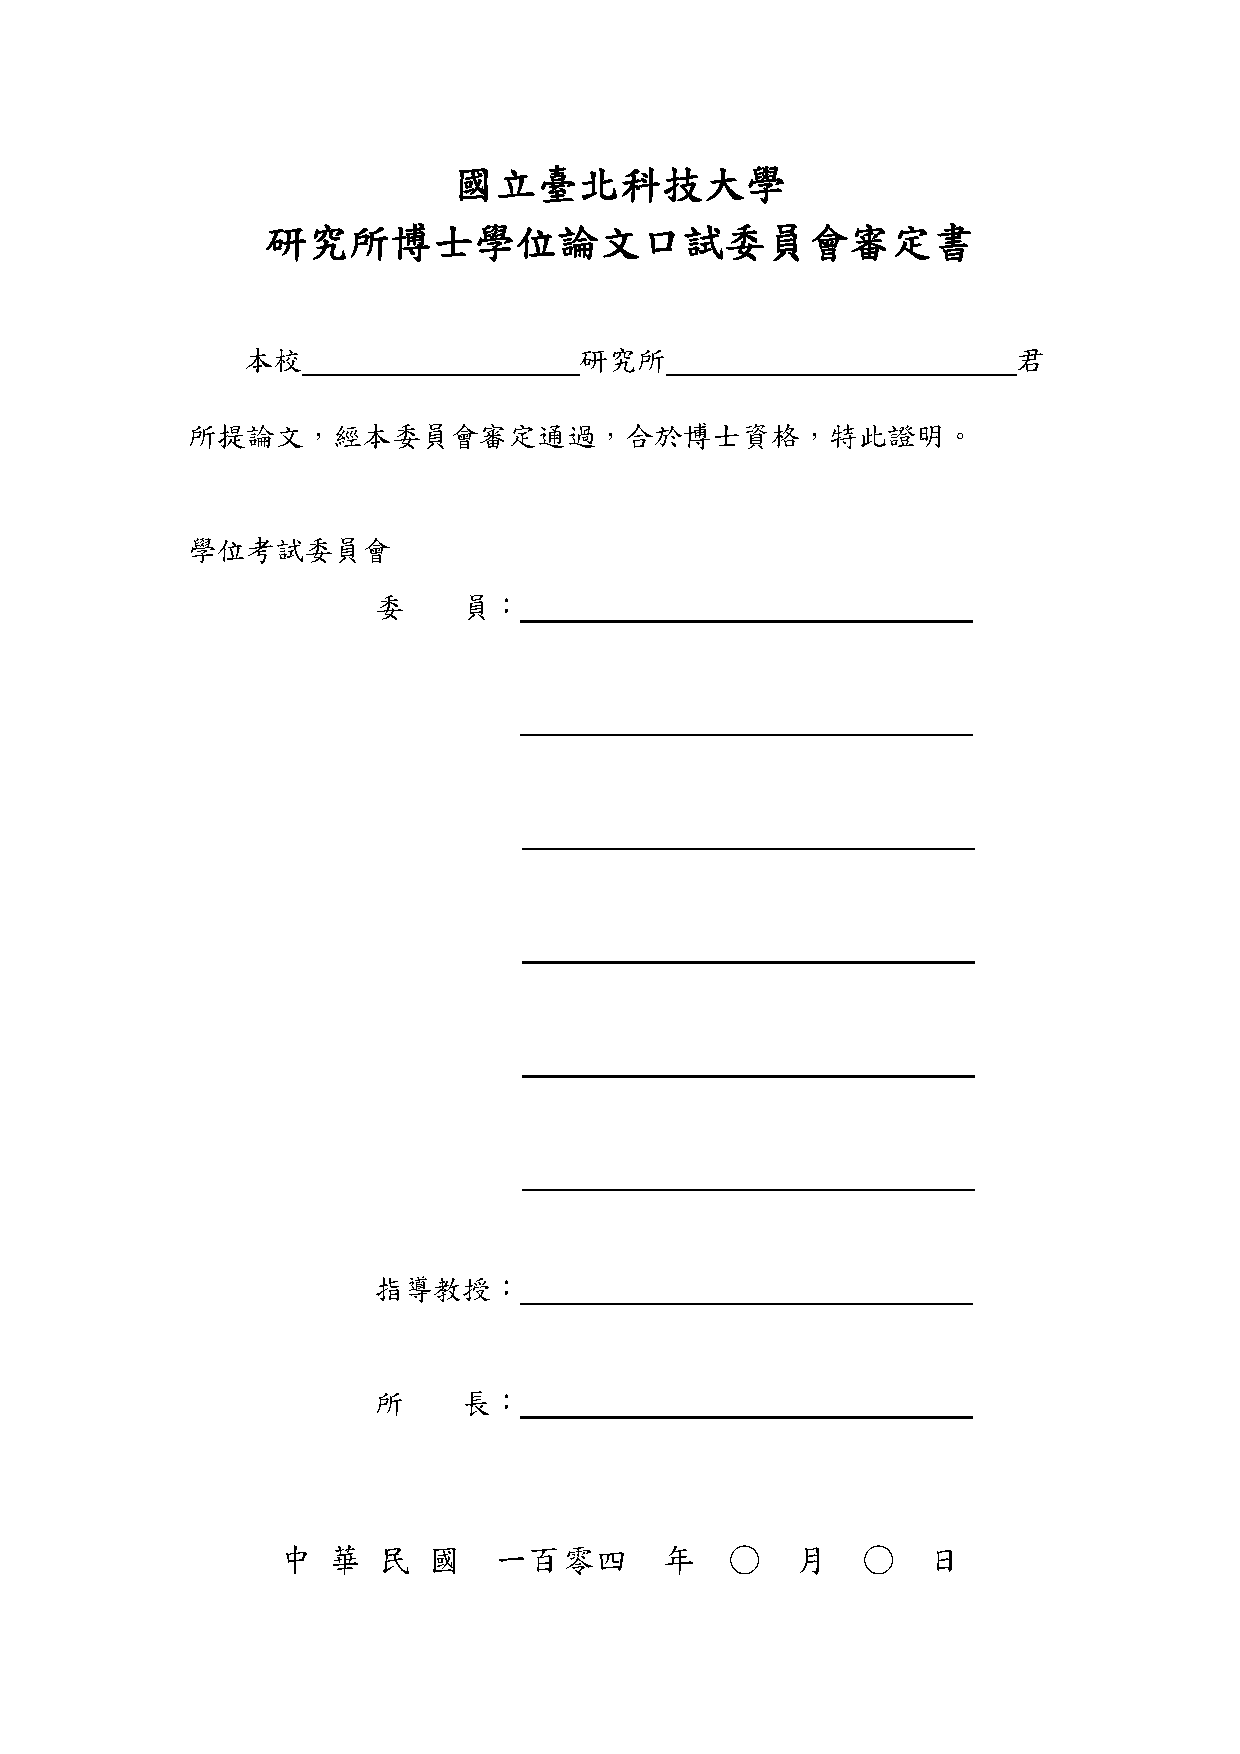
\includepdf{pdf/bb(18).pdf} % 轉檔案成 pdf
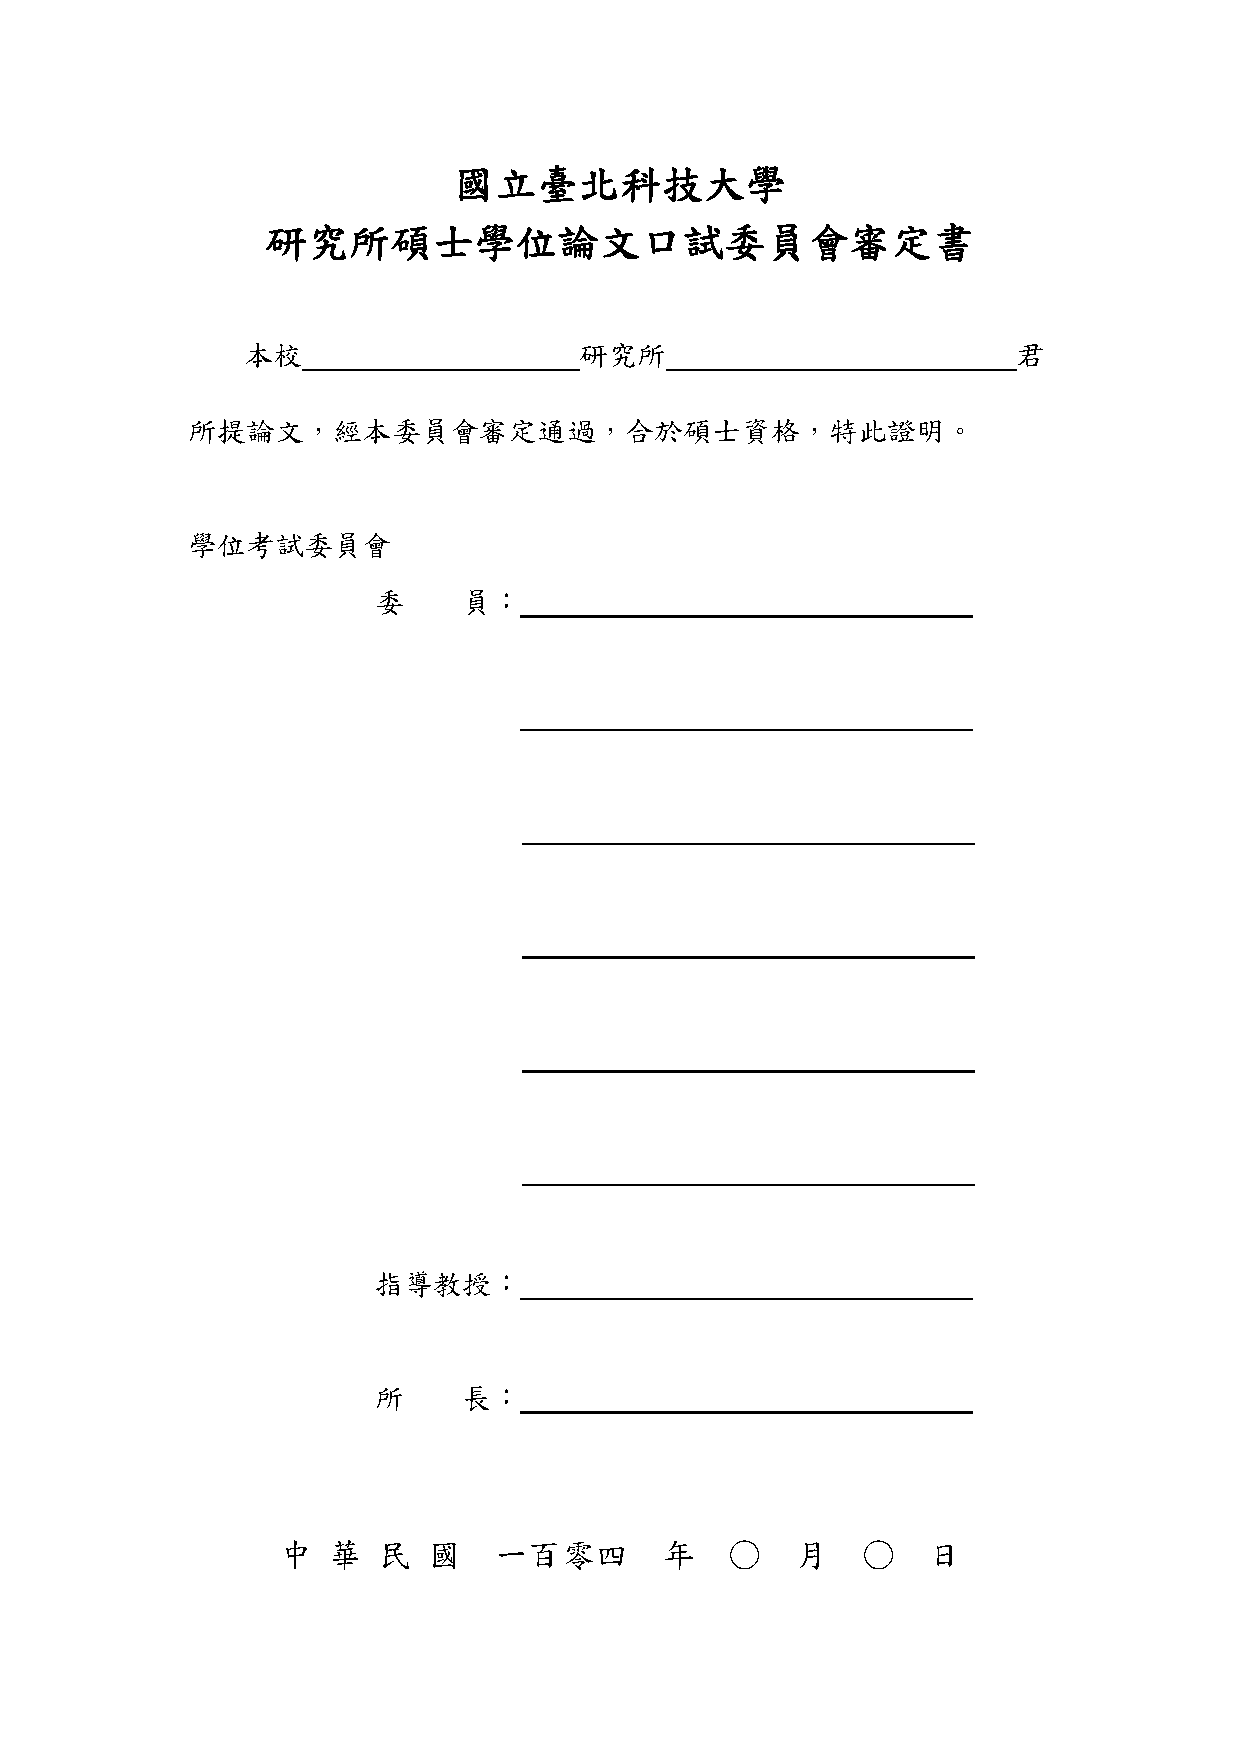
\includepdf{pdf/bb(19).pdf} % 轉檔案成 pdf

%\singlespacing
%\onehalfspacing
\doublespacing
\begin{abstractCH}

\noindent
論文名稱:機械元件設計之電腦輔助程式之發展\\
頁數:五十頁\\
校所別:國立臺北科技大學 電機工程  研究所\\
畢業時間:一百零一學年度 第一學期\\
學位:碩士\\
研究生:○○○\\
指導教授:姚立德 博士\\

\noindent
關鍵詞:機械元件、設計、電腦輔助程式\\

摘要為論文或報告的精簡概要,其目的是透過簡短的敘述使讀者大致瞭解整篇報告的內容。摘要的內容通常須包括問題的描述以及所得到的結果,但以不超過500字或一頁為原則,且不得有參考文獻或引用圖表等。以中文撰寫之論文除中文摘要外,得於中文摘要後另附英文摘要。標題使用20pt粗標楷體並於上、下方各空一行(1.5倍行高,字型12pt空行)後,鍵入摘要內容。摘要頁須編頁碼(小寫羅馬數字表示頁碼)。

\end{abstractCH}

\begin{abstractEN}

\noindent
Title: Development of Computer Aided Design of Mechanical Element\\
Pages: 50\\
School: National Taipei University of Technology\\
Department: Electrical Engineering\\
Time: June, 2012\\
Degree: Master\\
Researcher: Da-Ming Chen\\
Advisor: Li-De Yao, Ph.D.\\

\noindent
Keywords: Computer Aided Design, Mechanical Element\\


Start writing abstract from here. Start writing abstract from here. Start writing abstract from here. Start writing abstract from here. Start writing abstract from here. Start writing abstract from here. Start writing abstract from here. Start writing abstract from here.


\end{abstractEN}

\begin{acknowledgementsCH}

所有對於研究提供協助之人或機構,作者都可在誌謝中表達感謝之意。標題使用20pt粗標楷體,並於上、下方各空一行(1.5倍行高,字型12pt空行)後鍵入內容。致謝頁須編頁碼(小寫羅馬數字表示頁碼)。\\\\



\begin{enumerate}[leftmargin=0pt, topsep=0pt, itemsep=0pt, label=\Roman{*}.]

\item 此範本參考下列網站的資料:
\begin{enumerate}[topsep=0pt, itemsep=0pt, label=$\bullet$]
    \item \href{https://code.google.com/p/ntu-thesis-latex-template/}{台大碩博士論文LaTeX範本}
    \item \href{http://exciton.eo.yzu.edu.tw/~lab/latex/latex_note.html}{陳念波老師的元智大學論文樣板}
    \item \href{https://code.google.com/p/ntust-thesis/}{台灣科技大學同學編寫的碩博士論文Latex模板}
\end{enumerate}

\item 原作者參考並修改自下列網站的資料:
\begin{enumerate}[topsep=0pt, itemsep=0pt, label=$\bullet$]
    \item \href{http://www.csie.ntu.edu.tw/~tzhuan/www/resources/ntu/}{如何用 LaTeX 排版臺灣大學碩士論文}\\
    \textemdash 台灣大學論文\LaTeX\ 樣版原創者\href{http://www.csie.ntu.edu.tw/~tzhuan/www/}{黃子桓}的教學網頁
    \item \href{http://www.hitripod.com/blog/2012/05/latex-thesis-template-quick-reference/}{LaTeX 常用語法及論文範本}\\
    \textemdash \href{http://www.hitripod.com/blog/}{Hitripod}所修改的範本,這裡參考了許多他所寫的格式和內容
    \item \href{http://www.cc.ntu.edu.tw/chinese/epaper/0014/20100920_1404.htm}{使用LaTeX做出精美的論文}
    \item \href{http://www.hitripod.com/blog/2011/04/xetex-chinese-font-cjk-latex/}{XeTeX:解決 LaTeX 惱人的中文字型問題}
    \item \href{http://code.google.com/p/ntuthesis/}{台灣大學碩士、博士論文的Latex模板}\\   
\end{enumerate}

\end{enumerate}


%----------- Have a fractal fern? -----------
%\begin{pspicture}
%\psFern[scale=30,maxIter=100000,linecolor=Green]
%\end{pspicture}

\end{acknowledgementsCH} 

\singlespacing
\tableofcontents

\onehalfspacing
\listoffigures
\listoftables

\mainmatter

\doublespacing

%----------- Include/Input your thesis here -----------
%normal cite == \input

\chapter{導論}
\label{c:1}

%==========================================================================================
\section{第一階層子標題}

各階層子標題均應置於左側,並於其下方不空行。

本規範為一般性規範,各所得依其學術領域之慣用格式,訂定相關規範。本規範為一般性規範,各所得依其學術領域之慣用格式,訂定相關規範。本規範為一般性規範,各所得依其學術領域之慣用格式,訂定相關規範。本規範為一般性規範,各所得依其學術領域之慣用格式,訂定相關規範。本規範為一般性規範,各所得依其學術領域之慣用格式,訂定相關規範。本規範為一般性規範,各所得依其學術領域之慣用格式,訂定相關規範。本規範為一般性規範,各所得依其學術領域之慣用格式,訂定相關規範。本規範為一般性規範,各所得依其學術領域之慣用格式,訂定相關規範。本規範為一般性規範,各所得依其學術領域之慣用格式,訂定相關規範。本規範為一般性規範,各所得依其學術領域之慣用格式,訂定相關規範。本規範為一般性規範,各所得依其學術領域之慣用格式,訂定相關規範。本規範為一般性規範,各所得依其學術領域之慣用格式,訂定相關規範。本規範為一般性規範,各所得依其學術領域之慣用格式,訂定相關規範。

%==========================================================================================
\subsection{第二階層子標題}

第二階層子標題之內文。

%==========================================================================================
\subsubsection{第三階層子標題}

第三階層子標題之內文。



%==========================================================================================
\section{Figure}
\label{ss:Figure}
\begin{figure}[htpb!]
  \centering
    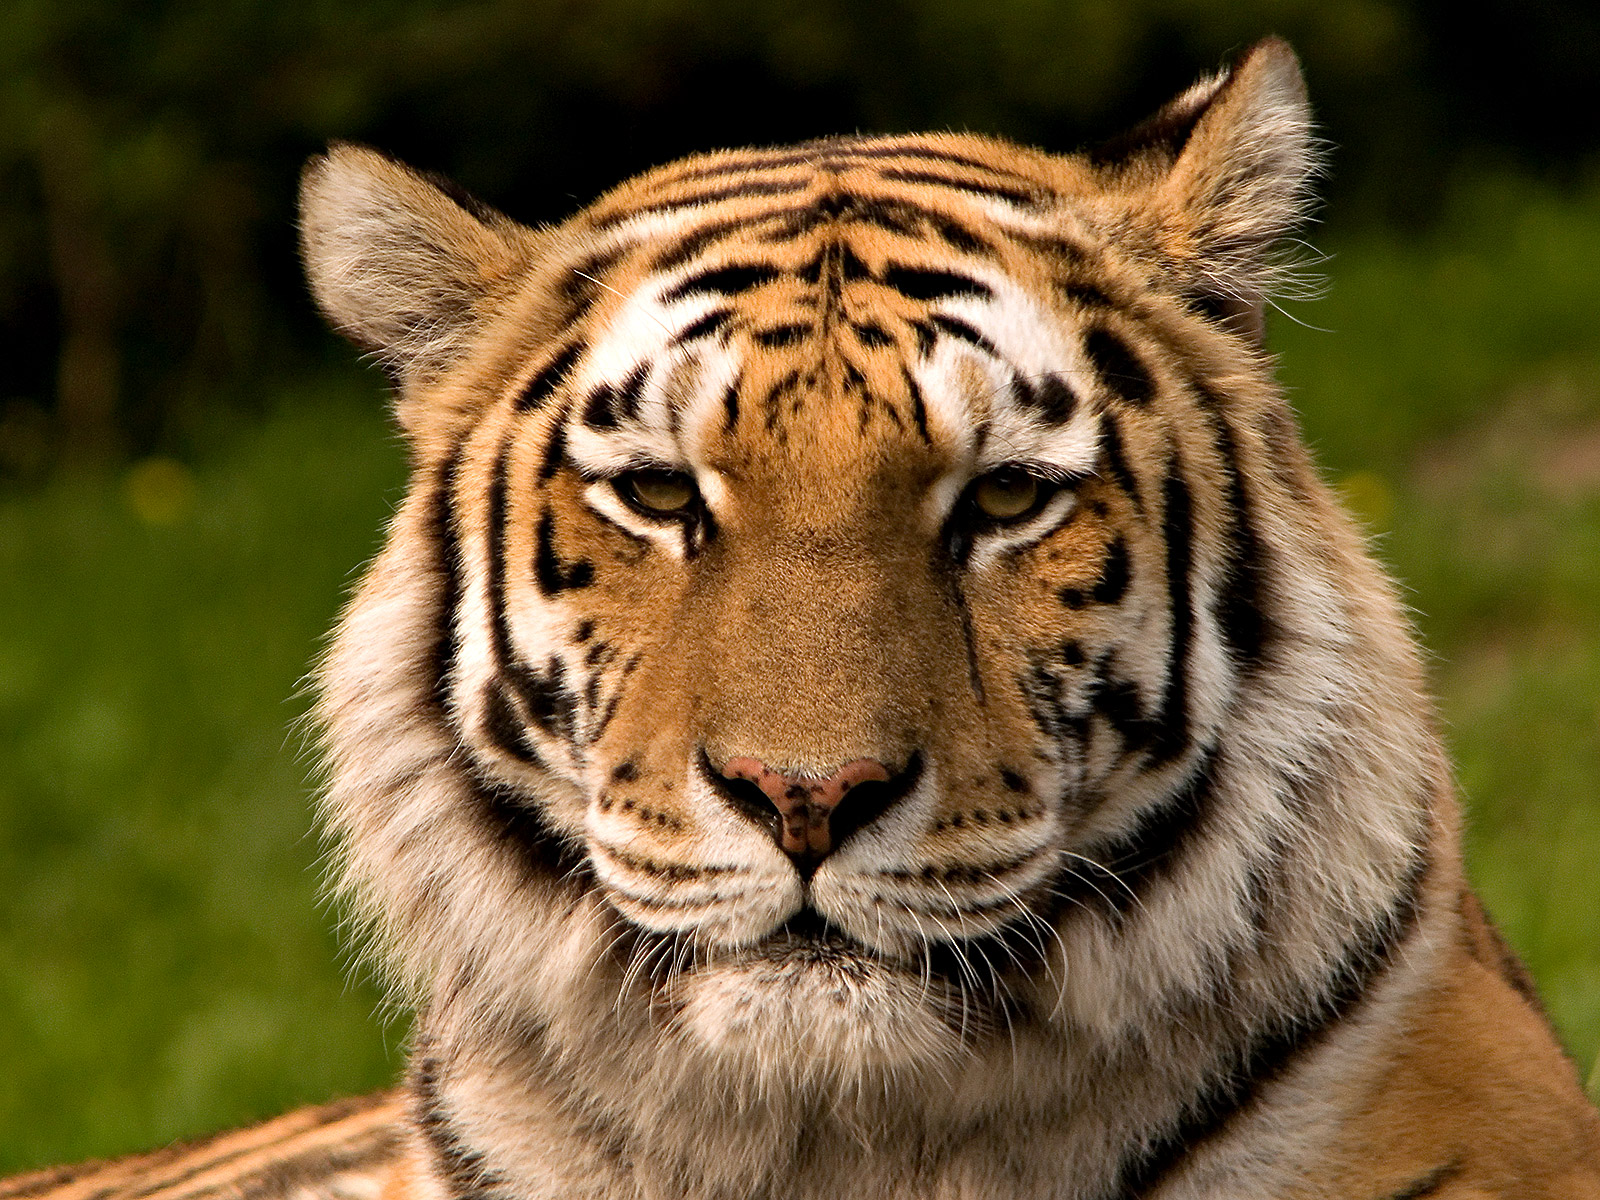
\includegraphics[width=0.5\textwidth]{fig/tiger.jpeg}
    \caption{\label{fig:tiger}A picture of a tiger.}
\end{figure}

Figure~\ref{fig:tiger} is a picture of a tiger.


% ntut



下圖\ref{fig:kamado}顯示的是 ``竈門炭治郎'' 的圖片。

\begin{figure}[h!]
    \centering
    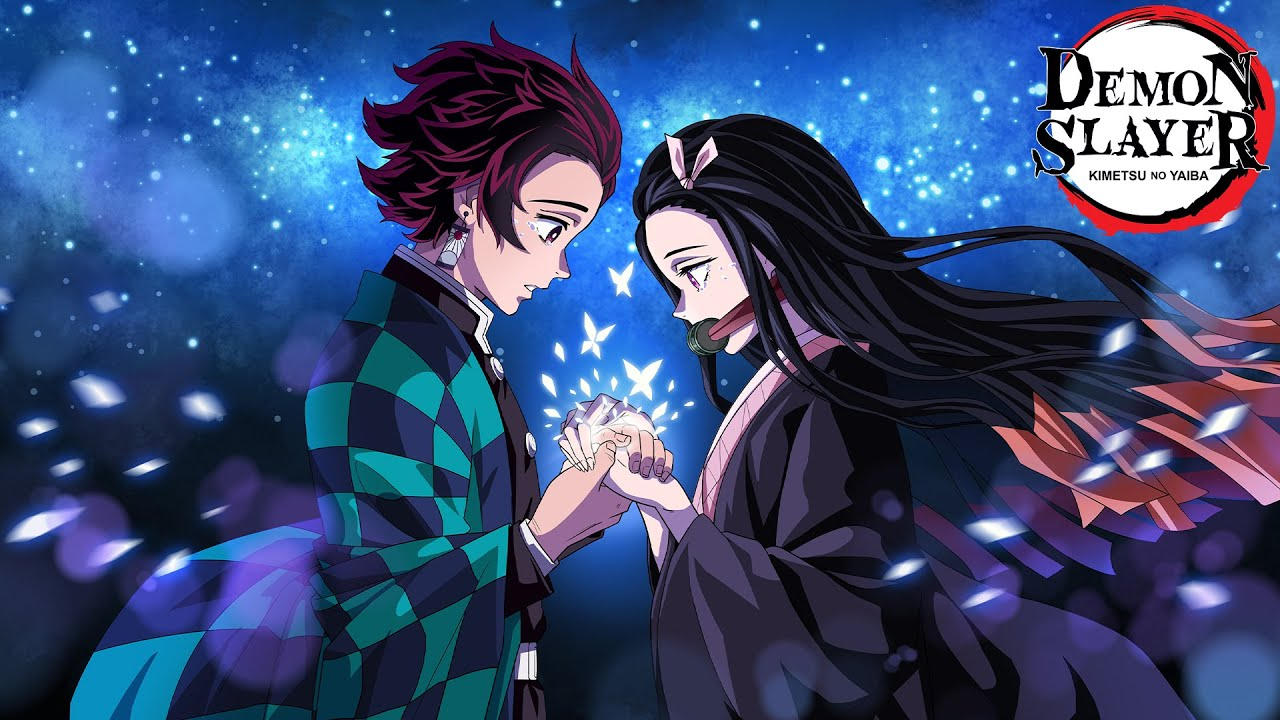
\includegraphics[width=0.85\textwidth]{fig/kamado/maxresdefault.jpg}
    \caption{這張圖片的說明, 竈門炭治郎。}
    \label{fig:kamado}
\end{figure}


竈門炭治郎的招式,是水之呼吸,見圖\ref{fig:kamado_ab}。圖\ref{fig:kamado_a}顯示的是 竈門炭治郎本人的圖片。圖\ref{fig:kamado_b}顯示的是 竈門炭治郎招式的圖片。


\begin{figure}[htbp]
\centering
\subfigure[我是圖a的說明]{
	
\includegraphics[width=0.22\textwidth]{fig/kamado/a.jpg}
	\label{fig:kamado_a}
}
\subfigure[我是圖b的說明]{
	
\includegraphics[width=0.22\textwidth]{fig/kamado/b.jpg}
	\label{fig:kamado_b}
}
\caption{我是整張圖a的說明}
\label{fig:kamado_ab}
\end{figure}



竈門炭治郎的招式,是水之呼吸,見圖\ref{fig:kamado_ab2}。圖\ref{fig:kamado_a2}顯示的是 竈門炭治郎本人的圖片。圖\ref{fig:kamado_b2}顯示的是 竈門炭治郎招式的圖片。圖\ref{fig:kamado_a3}顯示的是...。圖\ref{fig:kamado_b3}顯示的是...。



\begin{figure*}[htbp]
\centering
\subfigure[我是圖a的說明]{
	
\includegraphics[width=0.22\textwidth]{fig/kamado/a.jpg}
	\label{fig:kamado_a2}
}
\subfigure[我是圖b的說明]{
	
\includegraphics[width=0.22\textwidth]{fig/kamado/b.jpg}
	\label{fig:kamado_b2}
}
\subfigure[我是圖c的說明]{
	
\includegraphics[width=0.22\textwidth]{fig/kamado/a.jpg}
	\label{fig:kamado_a3}
}
\subfigure[我是圖d的說明]{
	
\includegraphics[width=0.22\textwidth]{fig/kamado/b.jpg}
	\label{fig:kamado_b3}
}
\caption{我是整張圖a的說明}
\label{fig:kamado_ab2}
\end{figure*}





中文缺字,。內文提到圖\ref{punica_compare}, Fig~\ref{punica_a}, Fig~\ref{punica_b}, Fig~\ref{punica_c}, Fig~\ref{punica_d}, Fig~\ref{punica_e}, Fig~\ref{punica_f}


\begin{figure}[htbp]
\centering
\subfigure[子圖a說明]{
	
\includegraphics[width=0.32\textwidth]{fig/flower/file(0).pdf}
	\label{punica_a}
}
\subfigure[子圖b說明]{
	
\includegraphics[width=0.32\textwidth]{fig/flower/file(1).pdf}
	\label{punica_b}
}
\subfigure[子圖c說明]{
	
\includegraphics[width=0.32\textwidth]{fig/flower/file(2).pdf}
	\label{punica_c}
}
\subfigure[子圖d說明]{
	
\includegraphics[width=0.32\textwidth]{fig/flower/file(3).pdf}
	\label{punica_d}
}
\subfigure[子圖e說明]{
	
\includegraphics[width=0.32\textwidth]{fig/flower/file(4).pdf}
	\label{punica_e}
}
\subfigure[子圖f說明]{
	
\includegraphics[width=0.32\textwidth]{fig/flower/file(4).pdf}
	\label{punica_f}
}
\caption{...}
\label{punica_compare}
\end{figure}




%==========================================================================================
\section{Table}
\label{ss:Table}

\href{http://en.wikibooks.org/wiki/LaTeX/Tables}{Table examples on WIKIBOOKS}.

\begin{table}[htpb]\begin{center}
\caption{Table Example 1}
\begin{tabularx}{8cm}{llX}
\hline
Start & End  & Character Block Name \\
\hline
3400  & 4DB5 & CJK Unified Ideographs Extension A \\
4E00  & 9FFF & CJK Unified Ideographs \\
\hline
\end{tabularx}
 \end{center}\end{table}

\begin{table}[htpb]\begin{center}
\caption{Table Example 2}
\begin{tabular}{llr}
\hline
\multicolumn{2}{c}{Item} \\
\cline{1-2}
Animal & Description & Price (\$) \\
\hline
Gnat  & per gram & 13.65 \\
      & each     &  0.01 \\
Gnu   & stuffed  & 92.50 \\
Emu   & stuffed  & 33.33 \\
Armadillo & frozen & 8.99 \\
\hline
\end{tabular}
 \end{center}\end{table}

 \begin{table}[htpb]\begin{center}
	\label{t:prefix-table}
	\caption{Table Example 3}
	\renewcommand{\arraystretch}{1.0}
	\begin{tabularx}{300pt}{|c|X| }
		\hline
		\multirow{1}{*}{\textbf{Allocation}} &
		Allocation, Element, Type, Script
		\\ \hline\hline
		%------------------------------
		\multirow{6}{*}{\textbf{Data Types}} &
        Byte2, Byte3, and Byte4\\ &
        Float2, Float3, Float4\\ &
        Int2, Int3, Int4\\ &
        Long2, Long3, Long4\\ &
        Matrix2f, Matrix3f, Matrix4f\\ &
        Short2, Short3, Short4
        \\ \hline\hline
		%------------------------------
		\multirow{4}{*}{\textbf{Graphics}} &
		Mesh\\&
		ProgramFragment, ProgramRaster\\&
		ProgramStore, ProgramVertex\\&
		RSSurfaceView
		\\ \hline
		%------------------------------
	\end{tabularx}
\end{center}\end{table}

\chapter{相關文獻討論}
\label{c:2}

%==========================================================================================
\section{第一階層子標題}

各階層子標題均應置於左側,並於其下方不空行。


fsdfdsdsaff f  ~\cite{Parker:2013}  fdsfgdsfdsg dfsf。

vdfvfdvfdvvdfv \cite{Hsiao:2018}


%==========================================================================================
\subsection{第二階層子標題}

第二階層子標題之內文。

%==========================================================================================
\subsubsection{第三階層子標題}

第三階層子標題之內文。


\chapter{方法}
\label{c:3}

%==========================================================================================
\section{第一階層子標題}

各階層子標題均應置於左側,並於其下方不空行。

%==========================================================================================
\subsection{第二階層子標題}

第二階層子標題之內文。

%==========================================================================================
\subsubsection{第三階層子標題}

第三階層子標題之內文。


%\bibliographystyle{unsrt}
%\bibliography{thesisbib} 
\chapter{結果與討論}
\label{c:4}

%==========================================================================================
\section{第一階層子標題}

各階層子標題均應置於左側,並於其下方不空行。

%==========================================================================================
\subsection{第二階層子標題}

第二階層子標題之內文。

%==========================================================================================
\subsubsection{第三階層子標題}

第三階層子標題之內文。


\chapter{結論}
\label{c:5}

%==========================================================================================
\section{結論}

各階層子標題均應置於左側,並於其下方不空行。

%==========================================================================================
\section{未來展望}

第二階層子標題之內文。


%\bibliographystyle{unsrt}
%\bibliography{thesisbib} 



%chapter cite  == \include

%\include{start}
%\include{introduction}
%\include{THM}
%\include{EXP}


%\appendix
%----------- Input your appendix here  -----------
%
% this file is encoded in utf-8
% v1.7
%%% 每一個附錄 (附錄一、附錄二、...) 都要複製此段附錄編排碼做為起頭
%%% 附錄編排碼 begin >>>
\newpage
\chapter*{附錄A:第一個附錄名稱} % 修改附錄編號與你的附錄名
\addcontentsline{toc}{chapter}{附錄A:第一個附錄名稱} %建議此內容應與上行相同
\renewcommand{\thechapter}{A} % 如果是附錄二,則內容應為{二}

\setcounter{equation}{0}
\setcounter{figure}{0}
\setcounter{footnote}{0}
\setcounter{section}{0}
\setcounter{subsection}{0}
\setcounter{subsubsection}{0}
\setcounter{table}{0}
%%% <<< 附錄編排碼 end



附錄內容
%
% this file is encoded in utf-8
% v1.7
%%% 每一個附錄 (附錄一、附錄二、...) 都要複製此段附錄編排碼做為起頭
%%% 附錄編排碼 begin >>>
\newpage
\chapter*{附錄B:第二個附錄名稱} % 修改附錄編號與你的附錄名
\addcontentsline{toc}{chapter}{附錄B:第二個附錄名稱} %建議此內容應與上行相同
\renewcommand{\thechapter}{B} % 如果是附錄二,則內容應為{二}

\setcounter{equation}{0}
\setcounter{figure}{0}
\setcounter{footnote}{0}
\setcounter{section}{0}
\setcounter{subsection}{0}
\setcounter{subsubsection}{0}
\setcounter{table}{0}
%%% <<< 附錄編排碼 end



附錄內容
%or %chapter cite  == \include
%%
% this file is encoded in utf-8
% v1.7
%%% 每一個附錄 (附錄一、附錄二、...) 都要複製此段附錄編排碼做為起頭
%%% 附錄編排碼 begin >>>
\newpage
\chapter*{附錄A:第一個附錄名稱} % 修改附錄編號與你的附錄名
\addcontentsline{toc}{chapter}{附錄A:第一個附錄名稱} %建議此內容應與上行相同
\renewcommand{\thechapter}{A} % 如果是附錄二,則內容應為{二}

\setcounter{equation}{0}
\setcounter{figure}{0}
\setcounter{footnote}{0}
\setcounter{section}{0}
\setcounter{subsection}{0}
\setcounter{subsubsection}{0}
\setcounter{table}{0}
%%% <<< 附錄編排碼 end



附錄內容
%%
% this file is encoded in utf-8
% v1.7
%%% 每一個附錄 (附錄一、附錄二、...) 都要複製此段附錄編排碼做為起頭
%%% 附錄編排碼 begin >>>
\newpage
\chapter*{附錄B:第二個附錄名稱} % 修改附錄編號與你的附錄名
\addcontentsline{toc}{chapter}{附錄B:第二個附錄名稱} %建議此內容應與上行相同
\renewcommand{\thechapter}{B} % 如果是附錄二,則內容應為{二}

\setcounter{equation}{0}
\setcounter{figure}{0}
\setcounter{footnote}{0}
\setcounter{section}{0}
\setcounter{subsection}{0}
\setcounter{subsubsection}{0}
\setcounter{table}{0}
%%% <<< 附錄編排碼 end



附錄內容

%
% this file is encoded in utf-8
% v1.7
%%% 每一個附錄 (附錄一、附錄二、...) 都要複製此段附錄編排碼做為起頭
%%% 附錄編排碼 begin >>>
\newpage
\chapter*{符號彙編}
\addcontentsline{toc}{chapter}{符號彙編}
\renewcommand{\thechapter}{符號彙編}

\setcounter{equation}{0}
\setcounter{figure}{0}
\setcounter{footnote}{0}
\setcounter{section}{0}
\setcounter{subsection}{0}
\setcounter{subsubsection}{0}
\setcounter{table}{0}
%%% <<< 附錄編排碼 end

\noindent
Symbol      Meaning\\
Θ			Debye's constant or characteristic temperature\\
Ω			efficiency; number of molecules\\
Ψ			availability of a closed system\\
Δ			internal energy (change) of reaction\\
Φ			availability of a closed system\\
ι			specific irreversibility\\
λ			critical state\\
μ			Joule-Thomson coefficient\\
ν			stoichiometric coefficient (number of moles in chemical equation)\\
ξ			cutoff ratio


\backmatter


%---------- Input your reference here ---------
\bibliographystyle{unsrt}
\addcontentsline{toc}{chapter}{\bibname}
\bibliography{thesis}

%----------- Input your Figure chapter here  -----------
%\input{EndFigTab}
%chapter cite  == \include
%\include{EndFigTab}

\end{document}
